\documentclass[a4paper,11pt]{article}
\usepackage[utf8]{inputenc}
\usepackage[T1]{fontenc}
\usepackage[ngerman]{babel}
\usepackage{amsmath,amssymb}
\usepackage{graphicx}
\usepackage{enumitem}
\usepackage{listings}
\usepackage{xcolor}
\usepackage{tikz}
\usepackage{pgf-umlcd}  % Add this line
\usepackage{hyperref}
\usepackage{booktabs}

\hypersetup{
    colorlinks=true,
    linkcolor=blue,
    filecolor=magenta,      
    urlcolor=cyan,
    pdftitle={CSV-Dateianalyse für Messdaten},
    pdfpagemode=FullScreen,
}

% Definiere Farben für Listings
\definecolor{codegreen}{rgb}{0,0.6,0}
\definecolor{codegray}{rgb}{0.5,0.5,0.5}
\definecolor{codepurple}{rgb}{0.58,0,0.82}
\definecolor{backcolour}{rgb}{0.95,0.95,0.92}

% Definiere C# als Sprache für Listings
\lstset{
    backgroundcolor=\color{backcolour},   
    commentstyle=\color{codegreen},
    keywordstyle=\color{magenta},
    numberstyle=\tiny\color{codegray},
    stringstyle=\color{codepurple},
    basicstyle=\ttfamily\footnotesize,
    breakatwhitespace=false,         
    breaklines=true,                 
    captionpos=b,                    
    keepspaces=true,                 
    numbers=left,                    
    numbersep=5pt,                  
    showspaces=false,                
    showstringspaces=false,
    showtabs=false,                  
    tabsize=2
}

\title{\textbf{Übung: CSV-Dateianalyse für Messdaten}}
\author{}
\date{}

\begin{document}

\maketitle
\tableofcontents
\newpage

\section{Einführung}
In dieser Übung entwickeln Sie eine Windows Forms-Anwendung in C\#, die CSV-Dateien mit Messdaten einlesen, anzeigen und auswerten kann. Die Anwendung soll die Anzahl der Messungen zählen und die durchschnittliche Messdauer berechnen. Diese Übung kombiniert Konzepte der Dateiverarbeitung, Datenanalyse und GUI-Programmierung.

\section{Lernziele}
Nach Abschluss dieser Übung sollten Sie in der Lage sein:
\begin{itemize}
    \item CSV-Dateien in C\# einzulesen und zu verarbeiten
    \item Daten in geeigneten Objektstrukturen zu speichern
    \item Einfache statistische Berechnungen durchzuführen
    \item Eine funktionale Windows Forms-Benutzeroberfläche zu erstellen
    \item Fehlerbehandlung in Dateioperationen zu implementieren
\end{itemize}

\section{Aufgabenbeschreibung}

\subsection{Benutzeroberfläche}
Erstellen Sie eine Windows Forms-Anwendung mit folgender Benutzeroberfläche:

\begin{figure}[htbp]
    \centering
    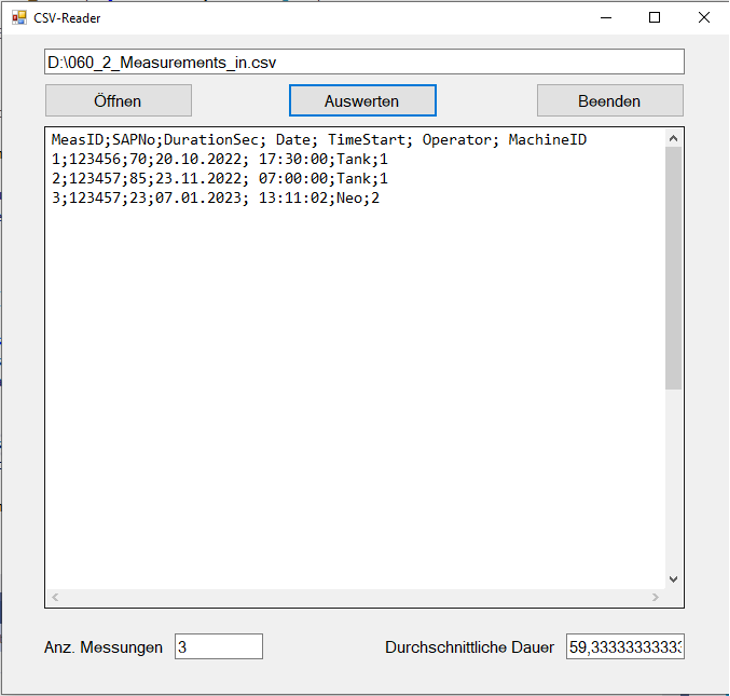
\includegraphics[width=0.8\textwidth]{screenshot.png}
    \caption{Beispiel der zu erstellenden Windows Forms-Benutzeroberfläche}
    \label{fig:screenshot}
\end{figure}

\begin{itemize}
    \item Eine Textbox zur Anzeige des Dateipfads (tbxFilepath)
    \item Drei Buttons:
    \begin{itemize}
        \item ``Öffnen'' (btnOpen): Zum Auswählen und Einlesen einer CSV-Datei
        \item ``Auswerten'' (btnAnalyze): Zur Analyse der eingelesenen Daten
        \item ``Beenden'' (btnExit): Zum Schließen der Anwendung
    \end{itemize}
    \item Eine große Textbox zur Anzeige des Dateiinhalts (tbxContent)
    \item Zwei Textboxen zur Anzeige der Auswertungsergebnisse:
    \begin{itemize}
        \item Anzahl der Messungen (tbxMeasurements)
        \item Durchschnittliche Messdauer (tbxAverageDuration)
    \end{itemize}
\end{itemize}


\subsection{Funktionalität}

\subsubsection{Öffnen-Button (btnOpen\_Click)}
\begin{enumerate}
    \item Öffnet einen Dateiauswahldialog (openFileDialog1)
    \item Liest bei erfolgreicher Auswahl die CSV-Datei ein
    \item Zeigt den Dateipfad in tbxFilepath an
    \item Überspringt die Kopfzeile der CSV-Datei
    \item Erstellt für jede Datenzeile ein Measurement-Objekt und fügt es einer Liste hinzu
    \item Zeigt den Inhalt der Liste in tbxContent an
\end{enumerate}

\subsubsection{Auswerten-Button (btnAnalyze\_Click)}
\begin{enumerate}
    \item Überprüft, ob die Datei eine gültige CSV-Datei ist (endet mit ``.csv'')
    \item Falls nicht, färbt die Textbox tbxFilepath rot und löscht die berechneten Werte
    \item Andernfalls:
    \begin{enumerate}
        \item Zählt die Anzahl der gültigen Messungen
        \item Berechnet die durchschnittliche Messdauer (DurationSec)
        \item Zeigt diese Werte in den entsprechenden Textboxen an
        \item Extrahiert und zeigt nur die MeasID und DurationSec-Werte in tbxContent an
    \end{enumerate}
\end{enumerate}

\subsubsection{Beenden-Button (btnExit\_Click)}
\begin{enumerate}
    \item Schließt die Anwendung mit Application.Exit()
\end{enumerate}

\section{Datenmodell}

\subsection{Measurement-Klasse}
Die Measurement-Klasse repräsentiert eine einzelne Messung aus der CSV-Datei. Sie enthält alle relevanten Daten und Methoden zur Verarbeitung dieser Daten.

\begin{center}
\begin{tikzpicture}
  \begin{class}[text width=11cm]{Measurement}{0,0}
    % Attributes section
    \attribute{- measId : int}
    \attribute{- SAPNo : int}
    \attribute{- durationSec : int}
    \attribute{- date : string}
    \attribute{- timeStart : string}
    \attribute{- op : string}
    \attribute{- machineId : int}
    \attribute{- startHour : int}
    \attribute{- startMinute : int}
    \attribute{- startSecond : int}
    
    % Methods section
    \operation{+ Measurement(csv : string)}
    \operation{+ Measurement(measId : int, SAPNo : int, durationSec : int, date : string, timeStart : string, op : string, machineId : int)}
    \operation{+ ToString() : string}
    \operation{+ ToCSV() : string}
    \operation{- ParseTimeStart() : void}
    \operation{+ GetTimeEnd() : string}
    \operation{+ ToCsvStartEnd() : string}
    \operation{+ GetDurationSec() : int}
  \end{class}
\end{tikzpicture}
\end{center}

\subsection{Detaillierte Beschreibung der Measurement-Klasse}

\subsubsection{Attribute}
\begin{itemize}
    \item \textbf{measId}: Eindeutige Identifikationsnummer der Messung
    \item \textbf{SAPNo}: SAP-Nummer des gemessenen Produkts
    \item \textbf{durationSec}: Dauer der Messung in Sekunden
    \item \textbf{date}: Datum der Messung im Format YYYY-MM-DD
    \item \textbf{timeStart}: Startzeit der Messung im Format HH:MM:SS
    \item \textbf{op}: Bezeichnung des Vorgangs/der Operation
    \item \textbf{machineId}: Identifikationsnummer der verwendeten Maschine
    \item \textbf{startHour, startMinute, startSecond}: Zerlegte Komponenten der Startzeit für Berechnungen
\end{itemize}

\subsubsection{Konstruktoren}
\begin{itemize}
    \item \textbf{Measurement(csv: string)}
    \begin{itemize}
        \item Erstellt ein Measurement-Objekt aus einer CSV-Zeile
        \item Zerlegt die durch Semikolon getrennte Zeichenkette in ihre Bestandteile
        \item Konvertiert die Werte in die entsprechenden Datentypen
        \item Speichert die Werte in den Attributen des Objekts
    \end{itemize}
    
    \item \textbf{Measurement(measId, SAPNo, durationSec, date, timeStart, op, machineId)}
    \begin{itemize}
        \item Erstellt ein Measurement-Objekt mit explizit angegebenen Werten
        \item Ermöglicht die manuelle Erstellung von Measurement-Objekten im Code
    \end{itemize}
\end{itemize}

\subsubsection{Methoden}
\begin{itemize}
    \item \textbf{ToString(): string}
    \begin{itemize}
        \item Überschreibt die Standard-ToString()-Methode
        \item Gibt eine formatierte Zeichenkette mit der Mess-ID und der Dauer zurück
        \item Format: ``\{measId\}: \{durationSec\}''
        \item Wird für die Anzeige in der Textbox verwendet
    \end{itemize}
    
    \item \textbf{ToCSV(): string}
    \begin{itemize}
        \item Konvertiert das Measurement-Objekt zurück in eine CSV-Zeile
        \item Verbindet alle Attribute mit Semikolons
        \item Nützlich für das Speichern von Daten zurück in eine CSV-Datei
    \end{itemize}
    
    \item \textbf{ParseTimeStart(): void} (private)
    \begin{itemize}
        \item Zerlegt die timeStart-Zeichenkette in Stunden, Minuten und Sekunden
        \item Speichert diese Werte in den entsprechenden Attributen
        \item Wird intern von GetTimeEnd() verwendet
    \end{itemize}
    
    \item \textbf{GetTimeEnd(): string}
    \begin{itemize}
        \item Berechnet die Endzeit der Messung basierend auf der Startzeit und der Dauer
        \item Ruft ParseTimeStart() auf, um die Startzeit zu zerlegen
        \item Addiert die Dauer in Sekunden zur Startzeit
        \item Berücksichtigt Überläufe bei Sekunden, Minuten und Stunden
        \item Gibt die Endzeit im Format HH:MM:SS zurück
    \end{itemize}
    
    \item \textbf{ToCsvStartEnd(): string}
    \begin{itemize}
        \item Erstellt eine CSV-Zeile mit Mess-ID, Startzeit und Endzeit
        \item Format: ``\{measId\};\{timeStart\};\{GetTimeEnd()\}''
        \item Nützlich für spezielle Auswertungen, die nur Start- und Endzeit benötigen
    \end{itemize}

    \item \textbf{GetDurationSec(): int}
    \begin{itemize}
        \item Gibt den Wert des durationSec-Attributs zurück
        \item Wird für die Berechnung der durchschnittlichen Messdauer verwendet
        \item Ermöglicht den Zugriff auf die private Variable durationSec von außerhalb der Klasse
    \end{itemize}

\end{itemize}

\subsection{Form1-Klasse}
Die Form1-Klasse implementiert die Benutzeroberfläche und die Logik zur Verarbeitung der CSV-Dateien.

\begin{center}
\begin{tikzpicture}
  % Form1-Klasse
  \begin{class}[text width=11cm]{Form1}{0,0}
    % Attributes section
    \attribute{- tbxFilepath : TextBox}
    \attribute{- btnOpen : Button}
    \attribute{- btnAnalyze : Button}
    \attribute{- btnExit : Button}
    \attribute{- tbxContent : TextBox}
    \attribute{- tbxMeasurements : TextBox}
    \attribute{- tbxAverageDuration : TextBox}
    \attribute{- openFileDialog1 : OpenFileDialog}
    \attribute{- measurements : List<Measurement>}
    
    % Methods section
    \operation{+ Form1()}
    \operation{- btnOpen\_Click(sender : object, e : EventArgs) : void}
    \operation{- btnAnalyze\_Click(sender : object, e : EventArgs) : void}
    \operation{- btnExit\_Click(sender : object, e : EventArgs) : void}
    \operation{- ReadCSVFile(filePath : string) : List<Measurement>}
    \operation{- CalculateAverageDuration() : double}
    \operation{- IsCSVFile(filePath : string) : bool}
    \operation{- DisplayMeasurements() : void}
  \end{class}
\end{tikzpicture}
\end{center}

\subsection{Beziehung zwischen den Klassen}
Die Form1-Klasse verwendet eine Liste von Measurement-Objekten zur Speicherung und Verarbeitung der eingelesenen Daten. Es handelt sich um eine unidirektionale Assoziation, da die Form1-Klasse die Measurement-Klasse kennt, aber nicht umgekehrt.

\subsection{Detaillierte Beschreibung der Form1-Klasse}

\subsubsection{Attribute}
\begin{itemize}
    \item \textbf{tbxFilepath}: Textbox zur Anzeige des Dateipfads
    \item \textbf{btnOpen}: Button zum Öffnen einer CSV-Datei
    \item \textbf{btnAnalyze}: Button zum Auswerten der Daten
    \item \textbf{btnExit}: Button zum Beenden der Anwendung
    \item \textbf{tbxContent}: Textbox zur Anzeige des Dateiinhalts
    \item \textbf{tbxMeasurements}: Textbox zur Anzeige der Anzahl der Messungen
    \item \textbf{tbxAverageDuration}: Textbox zur Anzeige der durchschnittlichen Messdauer
    \item \textbf{openFileDialog1}: Dialog zum Auswählen einer Datei
    \item \textbf{measurements}: Liste von Measurement-Objekten
\end{itemize}

\subsubsection{Methoden}
\begin{itemize}
    \item \textbf{Form1()}
    \begin{itemize}
        \item Konstruktor der Form1-Klasse
        \item Initialisiert die Komponenten der Benutzeroberfläche
    \end{itemize}
    
    \item \textbf{btnOpen\_Click(sender, e)}
    \begin{itemize}
        \item Ereignishandler für den Öffnen-Button
        \item Öffnet einen Dateiauswahldialog
        \item Liest die ausgewählte CSV-Datei ein
        \item Erstellt Measurement-Objekte und speichert sie in der Liste
        \item Zeigt den Inhalt in der Textbox an
    \end{itemize}
    
    \item \textbf{btnAnalyze\_Click(sender, e)}
    \begin{itemize}
        \item Ereignishandler für den Auswerten-Button
        \item Überprüft, ob die Datei eine gültige CSV-Datei ist
        \item Berechnet die Anzahl der Messungen und die durchschnittliche Messdauer
        \item Zeigt die Ergebnisse in den entsprechenden Textboxen an
    \end{itemize}
    
    \item \textbf{btnExit\_Click(sender, e)}
    \begin{itemize}
        \item Ereignishandler für den Beenden-Button
        \item Schließt die Anwendung
    \end{itemize}
    
    \item \textbf{ReadCSVFile(filePath)}
    \begin{itemize}
        \item Liest eine CSV-Datei ein und erstellt Measurement-Objekte
        \item Überspringt die Kopfzeile der CSV-Datei
        \item Gibt eine Liste von Measurement-Objekten zurück
    \end{itemize}
    
    \item \textbf{CalculateAverageDuration()}
    \begin{itemize}
        \item Berechnet die durchschnittliche Messdauer aller Measurement-Objekte
        \item Verwendet die GetDurationSec()-Methode der Measurement-Klasse
        \item Gibt den Durchschnittswert als double zurück
    \end{itemize}
    
    \item \textbf{IsCSVFile(filePath)}
    \begin{itemize}
        \item Überprüft, ob der angegebene Dateipfad auf eine CSV-Datei verweist
        \item Prüft, ob der Dateipfad mit ".csv" endet
        \item Gibt einen booleschen Wert zurück
    \end{itemize}
    
    \item \textbf{DisplayMeasurements()}
    \begin{itemize}
        \item Zeigt die Measurement-Objekte in der tbxContent-Textbox an
        \item Formatiert die Ausgabe gemäß den Anforderungen
    \end{itemize}
\end{itemize}


\section{Implementierungshinweise}

\subsection{CSV-Dateiformat}
Die zu verarbeitenden CSV-Dateien haben folgendes Format:
\begin{itemize}
    \item Die erste Zeile enthält Spaltenüberschriften
    \item Die Daten sind durch Semikolon (;) getrennt
    \item Jede Zeile repräsentiert eine Messung
\end{itemize}

\begin{verbatim}
MeasID;SAPNo;DurationSec;Date;TimeStart;OP;MachineID
1;12345;120;2023-01-01;10:15:00;Test;1
2;12346;180;2023-01-01;11:30:00;Test;2
\end{verbatim}

\subsection{Fehlerbehandlung}
Implementieren Sie folgende Fehlerbehandlungen:
\begin{itemize}
    \item Überprüfen Sie, ob die ausgewählte Datei mit ``.csv'' endet
    \item Färben Sie die Textbox mit dem Dateipfad rot, wenn es keine CSV-Datei ist
    \item Löschen Sie in diesem Fall die berechneten Werte
    \item Fangen Sie Ausnahmen bei der Dateiverarbeitung ab und zeigen Sie entsprechende Fehlermeldungen an
\end{itemize}

\subsection{Formatierung der Ausgabe}
\begin{itemize}
    \item Formatieren Sie die durchschnittliche Messdauer mit zwei Dezimalstellen
    \item Verwenden Sie für die Anzeige in tbxAverageDuration das Format ``\{0:0.00\}''
\end{itemize}

\section{Bewertungskriterien}
Ihre Lösung wird nach folgenden Kriterien bewertet:
\begin{itemize}
    \item Korrekte Implementierung der geforderten Funktionalität
    \item Saubere Strukturierung des Codes
    \item Angemessene Fehlerbehandlung
    \item Korrekte Berechnung der statistischen Werte
    \item Benutzerfreundliche Gestaltung der Benutzeroberfläche
\end{itemize}


\end{document}
